\documentclass[greek]{beamer}
%\usepackage{fontspec}
\usepackage{amsmath,amsthm}
\usepackage{unicode-math}
\usepackage{xltxtra}
\usepackage{graphicx}
\usetheme{CambridgeUS}
\usecolortheme{seagull}
\usepackage{hyperref}
\usepackage{ulem}
\usepackage{xgreek}
\usepackage{pgfpages}
\usepackage{tikz}
%\setbeameroption{show notes on second screen}
%\setbeameroption{show only notes}

\setsansfont{Noto Serif}

\usepackage{multicol}

% \newtheorem{definition}{Ορισμός}

\title{Συναρτήσεις}
\subtitle{Θεώρημα Bolzano}
\author[Λόλας]{Κωνσταντίνος Λόλας}
\date{}

\begin{document}

\begin{frame}
 \titlepage
\end{frame}

\section{Θεωρία}
\begin{frame}{Challenge}
 \begin{itemize}
  \item Φτιάξτε άξονες \pause
  \item Σημειώστε ένα σημείο $Α$ με θετική τεταγμένη και ένα σημείο $Β$ με αρνητική \pause
  \item Σχηματίστε συνάρτηση στο $[α,β]$ χωρίς να περάσετε από τον άξονα $x'x$ \pause
 \end{itemize}
 Συμπέρασμα...
\end{frame}

\begin{frame}{Χωρίς πολλά πολλά...}
 \begin{block}{Θεώρημα Bolzano}
  Έστω μια συνάρτηση $f$ ορισμένη σε κλειστό διάστημα $[α,β]$. Αν:
  \begin{itemize}
   \item η $f$ είναι συνεχής στο $[α,β]$ και
   \item $f(α)\cdot f(β)<0$,
  \end{itemize}
  τότε υπάρχει $x_0\in (α,β)$ τέτοιο ώστε $f(x_0)=0$
 \end{block}
\end{frame}

\begin{frame}{Παρατηρήσεις}
 \begin{itemize}
  \item ΔΕΝ είναι τρόπος επίλυσης εξισώσεων \pause
  \item ΔΕΝ βρίσκει - εντοπίζει ρίζες \pause
  \item ΔΕΝ τις μετράει σε πλήθος \pause
 \end{itemize}
 Το μόνο που κάνει είναι να σε πληροφορεί ότι ΣΙΓΟΥΡΑ έχει ρίζα μια συνάρτηση. \pause ΜΟΝΟ
\end{frame}

\begin{frame}{Τεστ μνήμης - ικανοτήτων}
 Πώς επιλύουμε εξισώσεις αλγεβρικά?
 \begin{itemize}
  \item Προφανής ρίζα \pause
  \item Λύνουμε ως προς $x$ \pause
  \item Παραγοντοποίηση \pause
  \item 1-1 \pause
 \end{itemize}
 Το μόνο που κάνει είναι να σε πληροφορεί ότι ΣΙΓΟΥΡΑ έχει ρίζα μια συνάρτηση. \pause ΜΟΝΟ
\end{frame}

\section{Ασκήσεις}
\begin{frame}{Εξάσκηση}
 Να αποδείξετε ότι:
 \begin{enumerate}
  \item Η συνάρτηση $f(x)=x^3+x-1$ ικανοποιεί τις υποθέσεις του θεωρήματος Bolzano στο διάστημα $[0,1]$.\pause
  \item Η εξίσωση $x^3+x-1=0$ έχει μία τουλάχιστον ρίζα στο διάστημα $(0,1)$.
 \end{enumerate}
\end{frame}

\begin{frame}{Εξάσκηση}
 Να αποδείξετε ότι υπάρχει ένα τουλάχιστον $x_0\in (0,1)$ τέτοιο ώστε $x_0^2+3x_0=e^{x_0}+1$.
\end{frame}

\begin{frame}{Εξάσκηση}
 Έστω $f:\mathbb{R}\to\mathbb{R}$ μία συνάρτηση η οποία είναι συνεχής με $f(\mathbb{R})=(0,1)$. Να αποδείξετε ότι η εξίσωση $f(x)=x-1$ έχει μία τουλάχιστον ρίζα στο διάστημα $(1,2)$.
\end{frame}

\begin{frame}{Εξάσκηση}
 Να αποδείξετε ότι η εξίσωση $\frac{e^x}{x-2}+\frac{x^2+1}{x-1}=0$ έχει μία τουλάχιστον ρίζα στο διάστημα $(1,2)$.
\end{frame}

\begin{frame}{Εξάσκηση}
 Να αποδείξετε ότι υπάρχει μοναδικό $x_0\in (0,1)$ τέτοιο ώστε $e^{x_0}+x_0=2$
\end{frame}

\begin{frame}{Εξάσκηση}
 Δίνονται οι συναρτήσεις $f(x)=\ln x$ και $g(x)=\frac{1}{x}$. Να αποδείξετε ότι οι $C_f$ και $C_g$ στο διάστημα $(1,e)$ έχουν ένα ακριβώς κοινό σημείο.
\end{frame}

\begin{frame}{Εξάσκηση}
 Να αποδείξετε ότι η εξίσωση $x^3-4x^2+2=0$ έχει δύο τουλάχιστον ρίζες στο διάστημα $(-1,1)$.
\end{frame}

\begin{frame}{Εξάσκηση}
 Δίνεται το ορθογώνιο $ΟΑΒΓ$ του σχήματος και μία συνεχής συνάρτηση $f$ στο $[0,2]$ της οποίας η γραφική παράσταση βρίσκεται στο χωρίο που ορίζει το ορθογώνιο. Να αποδείξετε ότι η $C_f$ τέμνει τη διαγώνιο $ΑΓ$.


 \centering
 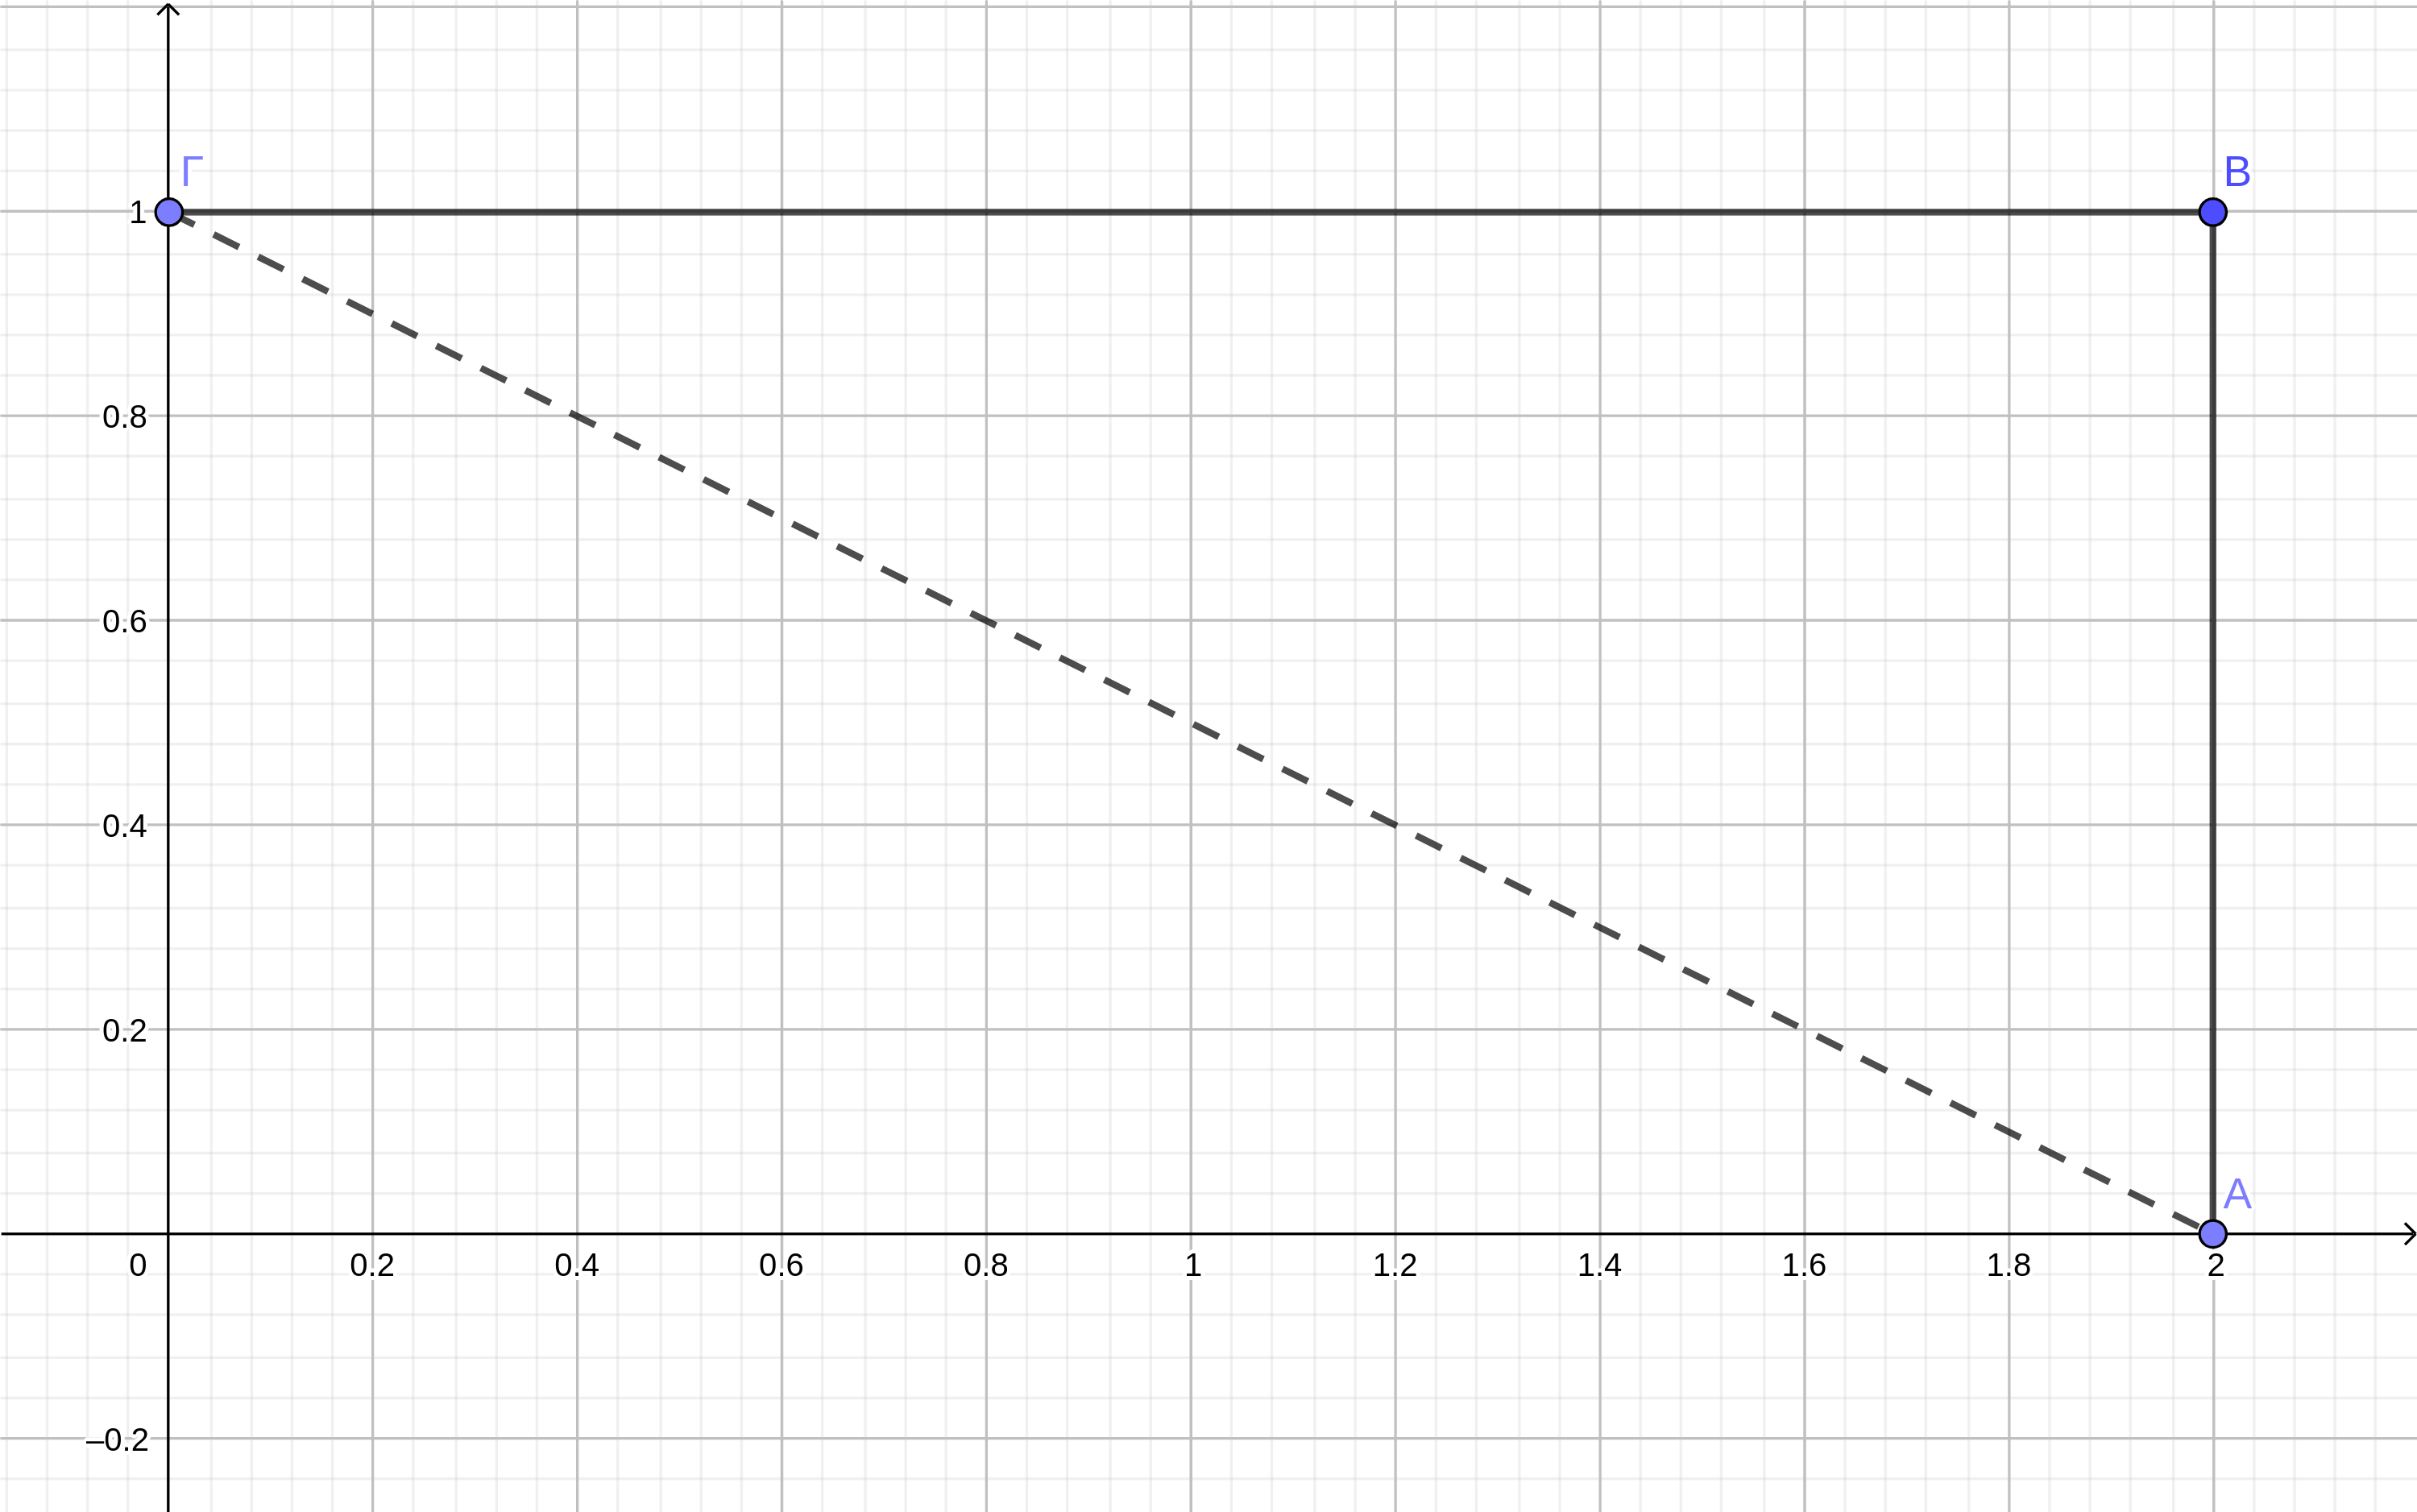
\includegraphics[width=0.5\textwidth]{"images/Bolzano.png"}
\end{frame}

\begin{frame}{Εξάσκηση}
 Να δείξετε ότι η εξίσωση $\ln x=\frac{1}{x-1}$ έχει μία τουλάχιστον ρίζα στο διάστημα $(0,1)$.
\end{frame}

\begin{frame}{Εξάσκηση}
  Έστω η συνεχής συνάρτηση $f:[0,1]\to\mathbb{R}$ με $-1<f(x)<0$, για κάθε $x\in [0,1]$. Να δείξετε ότι υπάρχει ένα τουλάχιστον $x_0\in (0,1)$ τέτοιο ώστε $f^2(x_0)=2f(x_0)+3x_0$
\end{frame}

\section{}
\begin{frame}
 Στο moodle θα βρείτε τις ασκήσεις που πρέπει να κάνετε, όπως και αυτή τη παρουσίαση
\end{frame}

\end{document}
